\subsection{Purpose}
The goal of this project is to design a game for 2 players, where the STM32’s microphone is used to control a robot, and the player who can defeat the opponent robot wins.\\*
This project is a variant of the project proposal where the STM32F4 was used in a game for 2 or more players to choose and recognise a frequency with the microphone.\\*
In our project, we use the embedded microphone of the board to controls the stepper motors and move the robot on the surrounding environment.

\subsection{Description of the robot}
The robot will have a cylindrical shape and it will be equipped with wheels on the bottom that will allow it to move forward, backward and rotate on itself.\\*
The engines that will allow the wheels to rotate are directly controlled by the STM32F4, the brain of our robot.
We will use 3D printer to build the body of the robot. 

\subsection{Game logic}
The game consists of a competition between 2 or more players. The players will control their robot through sounds, with the aim of attacking and overturning the opposing robot.\\*
A specific movement of the robot will correspond to each sound (frequency):
\begin{itemize}
	\item Forward movement
	\item Backward movement
	\item Rotation on itself
\end{itemize}
The rotation on itself is useful to turn around and attack the opposing robot

\subsection{Code structure}
We decided to structure the code in many components, in order to make the project extendable, easy to edit and easy to readapt.\\*
The main core of the robot is represented by the controller. All other components of the robot will be connected to the controller.\\*
The frequency analyser will convert the analog data obtained with the microphone into digital numbers.\\*
The controller will receive the information from the frequency analyser and it will use this information to directly control the wheels of the robot.

\newpage
\begin{figure}[h!]
	\hspace*{-0.15 \textwidth}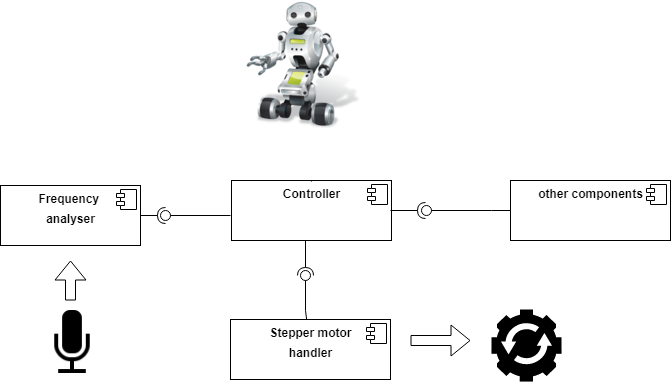
\includegraphics[width= 1.3\textwidth]
	{files/images/SystemStructure}
	\caption{This is a general overview of the system.}
\end{figure}